\documentclass[red]{beamer}
\usetheme{Warsaw}

% Fonts and encoding: pdfLaTeX needs inputenc/fontenc, LuaLaTeX and XeLaTeX use fontspec.
\usepackage{iftex}
\ifPDFTeX
    \usepackage[T1]{fontenc}
    \usepackage[utf8]{inputenc}
    \usepackage{lmodern}
\else
    \usepackage{fontspec}
\fi
\usepackage[polish]{babel}

\usepackage{graphicx}
\usepackage{booktabs}
\usepackage{listings}
\graphicspath{{../figs/}}

% No section navigation bar at the top and no navigation symbols.
\setbeamertemplate{headline}{}
\setbeamertemplate{navigation symbols}{}

\lstset{
    language=Python,
    basicstyle=\ttfamily\scriptsize,
    keywordstyle=\bfseries\color{red!60!black},
    commentstyle=\itshape\color{gray},
    stringstyle=\color{green!40!black},
    columns=fullflexible,
    keepspaces=true,
    showstringspaces=false,
    frame=single,
    rulecolor=\color{gray!50},
    xleftmargin=2pt,
    xrightmargin=2pt,
    aboveskip=2pt,
    belowskip=4pt,
}

\title[GHRS: miękkie metody klastrowania]{GHRS: Graph-based Hybrid Recommendation System with Application to Movie Recommendation}
\author[K. Kostka, R. Jarzyński, M. Jeżewski, M. Gagoś]{
    Kamil Kostka \and
    Radosław Jarzyński \and
    Maciej Jeżewski \and
    Michał Gagoś
}
\date{Lublin, \today}

\begin{document}

    \begin{frame}
    \titlepage
    \end{frame}

    \section{Artykuł bazowy}
    \begin{frame}{Artykuł bazowy}
        \small
        \begin{itemize}
            \item \textbf{Publikacja:} Darban i Valipour, \emph{Expert Systems with Applications}
                  (Elsevier, 2022), preprint arXiv:2111.11293
            \item \textbf{Idea GHRS:} graf podobieństwa użytkowników i dane demograficzne
                  $\rightarrow$ autoenkoder $\rightarrow$ K-Means $\rightarrow$ ocena jako
                  średnia w klastrze
            \item \textbf{Cel:} trafne rekomendacje przy zimnym starcie, czyli dla
                  użytkowników bez historii ocen
        \end{itemize}
        \begin{block}{Wynik deklarowany przez autorów (MovieLens 100K)}
            RMSE $= 0{,}887$, precyzja $0{,}771$, czułość $0{,}799$
        \end{block}
    \end{frame}

    \section{Audyt i Reprodukcja}
    \begin{frame}{Audyt i Reprodukcja}
        \small
        \begin{itemize}
            \item Autorzy udostępnili wyłącznie kod ekstrakcji cech (kroki 1-3)
            \item Autoenkoder (35-16-4-16-35), K-Means ($K = 8$) i Algorytm~1
                  odtworzyliśmy według opisu w artykule
            \item Ewaluacja: 5-krotna walidacja krzyżowa (u1-u5), 5 ziaren losowych,
                  graf budowany wyłącznie na danych treningowych
        \end{itemize}
        \begin{center}
            \begin{tabular}{lr}
                \toprule
                \textbf{Model} & \textbf{RMSE} \\
                \midrule
                GHRS: wynik z artykułu & $0{,}887$ \\
                GHRS: nasza reprodukcja & $1{,}076 \pm 0{,}001$ \\
                \bottomrule
            \end{tabular}
        \end{center}
        \begin{block}{Audyt}
            Zweryfikowaliśmy 13 hipotez dotyczących błędów ewaluacji, w tym wycieku
            danych testowych. Odtworzony potok stał się punktem odniesienia dla
            naszych rozszerzeń.
        \end{block}
    \end{frame}

    \section{Wkład Własny}
    \begin{frame}{Wkład Własny}
        \begin{block}{Proponowany tytuł artykułu}
            \centering\itshape
            Miękkie metody klastrowania (GMM, FCM) w~grafowo-hybrydowych systemach
            rekomendacyjnych zmagających się z~problemem zimnego startu
        \end{block}
        \footnotesize
        \begin{itemize}
            \item \textbf{Miękkie klastrowanie (GMM, FCM):} każdy użytkownik należy do
                  wszystkich $K$ klastrów z wagami sumującymi się do 1, a prognoza jest
                  wartością oczekiwaną średnich klaster-film
            \item \textbf{Reprezentacja generatywna (VAE):} wariacyjny autoenkoder zamiast
                  klasycznego, ciągła przestrzeń ukryta, optymalizator Nadam
            \item \textbf{Graf z TF-IDF:} krawędź wymaga podobnych ocen (próg $\alpha$)
                  oraz zbliżonego profilu gatunkowego (cosinus wektorów TF-IDF
                  $\geq 0{,}95$)
            \item \textbf{Ewaluacja:} 8 wariantów i 5 wariantów kontrolnych na tych samych
                  foldach i ziarnach; testy sparowane z poprawką Nadeau i Bengio oraz
                  korektą Holma
        \end{itemize}
    \end{frame}

    \begin{frame}[fragile]{Fragmenty implementacji}
        \footnotesize
        Miękkie przypisanie w algorytmie FCM (\texttt{ghrs/clustering\_soft.py}):
\begin{lstlisting}
def _fcm_weights(d2: np.ndarray, m: float) -> np.ndarray:
    logw = -np.log(np.maximum(d2, 1e-12)) / (m - 1.0)
    w = np.exp(logw - logw.max(axis=1, keepdims=True))
    return w / w.sum(axis=1, keepdims=True)
\end{lstlisting}
        Prawdopodobieństwa a posteriori w modelu GMM (ten sam moduł):
\begin{lstlisting}
gm = GaussianMixture(n_components=k, ...).fit(X)
p = gm.predict_proba(X)
\end{lstlisting}
        VAE: Nadam i reparametryzacja (\texttt{ghrs/autoencoder\_vae.py}):
\begin{lstlisting}
optimizer: str = "nadam"
...
eps = keras.random.normal(ops.shape(z_mean), seed=self.seed_generator)
return z_mean + ops.exp(0.5 * z_log_var) * eps
\end{lstlisting}
    \end{frame}

    \section{Wyniki}
    \begin{frame}{Wyniki: porównanie RMSE}{MovieLens 100K, 5-krotna walidacja krzyżowa (u1-u5)}
        \begin{center}
            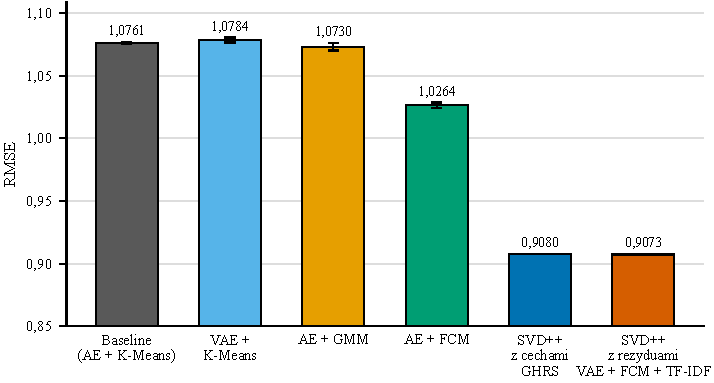
\includegraphics[width=0.85\textwidth]{fig1_rmse_comparison.pdf}
        \end{center}
        \small
        \begin{itemize}
            \item \textbf{FCM obniża RMSE} z $1{,}076$ do $1{,}026$: poprawa o $0{,}050$
                  we wszystkich 5 foldach ($p < 0{,}001$)
            \item GMM: $1{,}073$; VAE z K-Means: $1{,}079$
        \end{itemize}
    \end{frame}

    \begin{frame}{Wyniki: wpływ współczynnika rozmycia}{MovieLens 100K, model AE + FCM}
        \begin{center}
            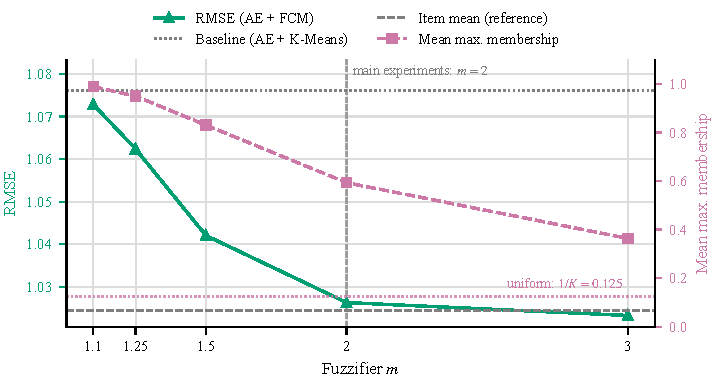
\includegraphics[width=0.85\textwidth]{fig2_fuzziness.pdf}
        \end{center}
        \small
        \begin{itemize}
            \item Wraz ze wzrostem $m$ maleją zarówno maksymalne wagi przynależności,
                  jak i RMSE: z $1{,}073$ ($m = 1{,}1$) do $1{,}023$ ($m = 3$)
            \item Miękkie przypisanie działa jak regularyzacja: uśrednia szum
                  pojedynczych klastrów
        \end{itemize}
    \end{frame}

    \begin{frame}{Wyniki: zimny start}{MovieLens 100K}
        \small
        10\% użytkowników bez ocen treningowych, 3 losowania:
        \begin{center}
            \begin{tabular}{lrr}
                \toprule
                \textbf{Model} & \textbf{RMSE} & \textbf{Zmiana} \\
                \midrule
                AE + K-Means (reprodukcja) & $1{,}133$ & \\
                VAE + K-Means & $1{,}138$ & $+0{,}005$ \\
                Graf TF-IDF + AE + K-Means & $1{,}115$ & $-0{,}018$ \\
                AE + FCM & $1{,}030$ & $-0{,}103$ \\
                VAE + FCM + TF-IDF & $1{,}031$ & $-0{,}102$ \\
                \bottomrule
            \end{tabular}
        \end{center}
        \begin{itemize}
            \item \textbf{FCM zmniejsza błąd dla nowych użytkowników} o $0{,}10$
                  we wszystkich losowaniach
            \item VAE i graf TF-IDF zastosowane samodzielnie zmieniają wynik nieznacznie
        \end{itemize}
    \end{frame}

    \section{Podsumowanie}
    \begin{frame}{Podsumowanie i kod źródłowy}
        \small
        \begin{itemize}
            \item Odtworzyliśmy pełny potok GHRS i przeprowadziliśmy jego audyt na zbiorze
                  MovieLens 100K: RMSE $1{,}076$ wobec deklarowanych $0{,}887$
            \item Miękkie klastrowanie FCM obniża RMSE do $1{,}026$, a przy zimnym
                  starcie zmniejsza błąd o $0{,}10$
            \item Zidentyfikowaliśmy mechanizm poprawy: regularyzację przez miękkie
                  przypisanie do klastrów
            \item Dalsze prace: dobór $K$ i $m$ na zbiorze walidacyjnym; wstępnie,
                  dla $K = 2$ FCM osiąga $1{,}023$
        \end{itemize}
        \begin{block}{Kod źródłowy (otwarty i w pełni odtwarzalny)}
            \url{https://github.com/KaloeSan/ghrs-soft-clustering}\\[2pt]
            Python 3.14, PyTorch, scikit-learn; wszystkie wyniki i wykresy generowane
            skryptami
        \end{block}
    \end{frame}

\end{document}
